\documentclass{article}
\usepackage{amsmath}
\usepackage{tikz}
\usepackage[paperwidth=18cm,paperheight=11.6cm,margin=0cm,noheadfoot]{geometry}
\usetikzlibrary{arrows.meta,calc,positioning}
\setlength{\parindent}{0pt}
\pagestyle{empty}

\definecolor{ink}{HTML}{202832}
\definecolor{muted}{HTML}{5F6C78}
\definecolor{rule}{HTML}{A5B0BA}
\definecolor{navy}{HTML}{164B73}
\definecolor{blue}{HTML}{1677C8}
\definecolor{cyan}{HTML}{00A6A6}
\definecolor{teal}{HTML}{16877D}
\definecolor{green}{HTML}{3B8F55}
\definecolor{orange}{HTML}{F28C28}
\definecolor{violet}{HTML}{7B4FC6}
\definecolor{coral}{HTML}{E45B5B}

\tikzset{
  flow/.style={draw=ink, line width=1.15pt,
               -{Latex[length=2.5mm,width=1.8mm]}},
  softflow/.style={draw=muted, line width=.9pt,
                   -{Latex[length=2.2mm,width=1.6mm]}},
  panel/.style={draw=rule, fill=white, line width=.9pt,
                rounded corners=2.5pt},
  card/.style={draw=ink, fill=white, line width=1pt,
               rounded corners=2pt, align=center,
               font=\sffamily\bfseries\fontsize{13}{15}\selectfont,
               text=ink},
  note/.style={draw=rule, fill=black!2, line width=.75pt,
               rounded corners=2pt, align=center,
               font=\sffamily\fontsize{11.5}{13.5}\selectfont,
               text=ink},
  title/.style={anchor=west, text=ink,
                font=\sffamily\bfseries\fontsize{18}{20}\selectfont},
  small/.style={text=muted, font=\sffamily\fontsize{11}{13}\selectfont}
}

\newcommand{\pagetitle}[1]{%
  \node[title] at (0.35,10.88) {#1};
}

\newcommand{\accentcard}[7]{%
  \node[card, draw=#6, fill=#6!11, minimum width=#3cm,
        minimum height=#4cm, text width=\dimexpr#3cm-8pt\relax,
        anchor=center] (#7) at (#1,#2) {#5};
}

\begin{document}

% Page 1: inverse model

\begin{tikzpicture}[remember picture,overlay,x=1cm,y=1cm]
\begin{scope}[shift={(current page.south west)}]
  \pagetitle{Inverse dynamics network (ID)}
  \node[panel, minimum width=3.1cm, minimum height=7.45cm,
        anchor=south west] at (0.38,1.65) {};
  \node[anchor=center, font=\sffamily\bfseries\fontsize{8}{9.5}\selectfont,
        text=navy] at (1.93,8.70) {Normalised inputs - 28};
  \accentcard{1.93}{7.35}{2.35}{1.18}{State\\[-1pt]\normalfont 16}{blue}{idstate}
  \accentcard{1.93}{5.38}{2.35}{1.18}{Desired motion\\[-1pt]\normalfont 8}{violet}{idtarget}
  \accentcard{1.93}{3.40}{2.35}{1.18}{Previous valve\\[-1pt]\normalfont 4}{orange}{idhistory}
  \accentcard{4.90}{5.38}{2.15}{2.05}{Input\\projection\\[-1pt]\normalfont $28\rightarrow512$}{navy}{idproj}
  \coordinate (idjoin) at (3.53,5.38);
  \draw[draw=ink, line width=1.15pt] (idstate.east) -| (idjoin);
  \draw[draw=ink, line width=1.15pt] (idtarget.east) -- (idjoin);
  \draw[draw=ink, line width=1.15pt] (idhistory.east) -| (idjoin);
  \draw[flow] (idjoin) -- (idproj.west);
  \accentcard{8.65}{5.38}{4.65}{2.75}
    {Four residual blocks\\[3pt]
     \normalfont\fontsize{11.5}{13.5}\selectfont
     LayerNorm $\rightarrow$ Linear $\rightarrow$ SiLU\\
     Dropout $\rightarrow$ Linear $+$ skip}{blue}{idtrunk}
  \draw[flow] (idproj.east) -- (idtrunk.west);
  \draw[draw=blue, line width=1pt, -{Latex[length=2.2mm,width=1.6mm]}]
    ($(idtrunk.north west)+(0.45,0.12)$) .. controls +(0,0.48) and +(0,0.48) ..
    ($(idtrunk.north east)+(-0.45,0.12)$);
  \node[small, font=\sffamily\fontsize{10}{12}\selectfont, anchor=south]
    at (8.65,7.48) {identity skip path};
  \accentcard{12.65}{5.38}{2.05}{2.05}{Output head\\[-1pt]\normalfont $512\rightarrow4$}{cyan}{idout}
  \draw[flow] (idtrunk.east) -- (idout.west);
  \accentcard{15.60}{5.38}{1.65}{1.42}{$\Delta\boldsymbol{u}_k$}{cyan}{iddu}
  \draw[flow] (idout.east) -- (iddu.west);
  \node[note, draw=orange, fill=orange!8, minimum width=4.1cm,
        minimum height=1.05cm] (idaccumulate) at (15.60,2.10)
    {accumulate $+$ per-axis clip};
  \draw[softflow] (iddu.south) -- (idaccumulate.north);
\end{scope}
\end{tikzpicture}
\null\newpage

% Page 2: forward model

\begin{tikzpicture}[remember picture,overlay,x=1cm,y=1cm]
\begin{scope}[shift={(current page.south west)}]
  \pagetitle{Forward dynamics network (FD)}
  \node[panel, minimum width=3.25cm, minimum height=7.35cm,
        anchor=south west] at (0.40,1.65) {};
  \node[anchor=west, font=\sffamily\bfseries\fontsize{9.5}{11.5}\selectfont,
        text=teal] at (0.70,8.60) {Causal inputs - 20};
  \accentcard{2.02}{7.05}{2.45}{1.30}{Valve command\\[-1pt]\normalfont $\boldsymbol{u}_k$ - 4}{teal}{fdvalve}
  \accentcard{2.02}{3.75}{2.45}{1.65}{Cylinder state\\[-1pt]\normalfont $\boldsymbol{x},\dot{\boldsymbol{x}},\Delta\boldsymbol{p},\boldsymbol{F}$\\16}{blue}{fdstate}
  \accentcard{4.85}{5.40}{2.05}{2.05}{Input\\projection\\[-1pt]\normalfont $20\rightarrow512$}{navy}{fdproj}
  \coordinate (fdjoin) at (3.55,5.40);
  \draw[draw=ink, line width=1.15pt] (fdvalve.east) -| (fdjoin);
  \draw[draw=ink, line width=1.15pt] (fdstate.east) -| (fdjoin);
  \draw[flow] (fdjoin) -- (fdproj.west);
  \accentcard{8.30}{5.40}{4.10}{2.65}
    {Shared residual\\trunk\\[3pt]
     \normalfont\fontsize{11.5}{13.5}\selectfont
     $4\times$ pre-norm blocks\\
     width 512 $+$ skip}{teal}{fdtrunk}
  \draw[flow] (fdproj.east) -- (fdtrunk.west);
  \accentcard{12.00}{5.40}{1.95}{2.05}{Output\\projection\\[-1pt]\normalfont $512\rightarrow12$}{navy}{fdout}
  \draw[flow] (fdtrunk.east) -- (fdout.west);
  \accentcard{15.35}{7.55}{2.35}{1.05}{$\Delta\hat{\boldsymbol{x}}$ - 4}{green}{fdx}
  \accentcard{15.35}{5.40}{2.35}{1.05}{$\Delta\hat{\dot{\boldsymbol{x}}}$ - 4}{blue}{fdv}
  \accentcard{15.35}{3.25}{2.35}{1.05}{$\Delta\widehat{\Delta\boldsymbol{p}}$ - 4}{violet}{fdp}
  \coordinate (fdsplit) at (13.50,5.40);
  \draw[flow] (fdout.east) -- (fdsplit) |- (fdx.west);
  \draw[flow] (fdsplit) -- (fdv.west);
  \draw[flow] (fdsplit) |- (fdp.west);
\end{scope}
\end{tikzpicture}
\null\newpage

% Page 3: ROM

\begin{tikzpicture}[remember picture,overlay,x=1cm,y=1cm]
\begin{scope}[shift={(current page.south west)}]
  \pagetitle{Command-conditioned hydraulic ROM}
  \node[panel, minimum width=17.25cm, minimum height=3.85cm,
        anchor=south west] at (0.37,6.00) {};
  \node[anchor=west, font=\sffamily\bfseries\fontsize{13}{15}\selectfont,
        text=navy] at (0.68,9.50) {1. Neural proposal};
  \accentcard{1.70}{7.75}{2.35}{1.55}{History\\[-1pt]\normalfont $6\times24$ rows\\$0.25$ s}{blue}{romhist}
  \accentcard{4.40}{7.75}{2.15}{1.55}{Two-layer GRU\\[-1pt]\normalfont $24\rightarrow128$}{blue}{romgru}
  \accentcard{6.85}{7.75}{1.45}{1.35}{Latent\\[-1pt]$\boldsymbol{h}_k$}{navy}{romlatent}
  \draw[flow] (romhist.east) -- (romgru.west);
  \draw[flow] (romgru.east) -- (romlatent.west);
  \accentcard{9.25}{7.75}{2.20}{1.15}{\fontsize{12}{14}\selectfont Actuation\\head}{orange}{romact}
  \accentcard{12.20}{7.75}{2.35}{1.15}{\fontsize{12}{14}\selectfont Bounded\\residuals}{violet}{romres}
  \accentcard{15.15}{7.75}{2.20}{1.15}{\fontsize{12}{14}\selectfont Load\\head}{teal}{romload}
  \coordinate (rombus) at (8.05,8.80);
  \draw[draw=ink, line width=1.15pt] (romlatent.east) -- (8.05,7.75) -- (rombus) -- (15.15,8.80);
  \draw[flow] (9.25,8.80) -- (romact.north);
  \draw[flow] (12.20,8.80) -- (romres.north);
  \draw[flow] (15.15,8.80) -- (romload.north);
  \node[panel, minimum width=17.25cm, minimum height=4.15cm,
        anchor=south west] at (0.37,1.00) {};
  \node[anchor=west, font=\sffamily\bfseries\fontsize{13}{15}\selectfont,
        text=green] at (0.68,4.78) {2. Explicit hydraulic update};
  \accentcard{1.95}{2.65}{2.55}{1.42}{Orifice flow}{green}{romflow}
  \accentcard{5.15}{2.65}{2.55}{1.42}{Pressure\\continuity}{green}{rompressure}
  \accentcard{8.35}{2.65}{2.35}{1.42}{Cylinder force\\[-1pt]\normalfont $\Delta p A$}{green}{romforce}
  \accentcard{11.45}{2.65}{2.35}{1.42}{Velocity\\dynamics}{green}{romvelocity}
  \accentcard{14.70}{2.65}{2.45}{1.42}{Position\\integration}{green}{romposition}
  \draw[flow] (romflow.east) -- (rompressure.west);
  \draw[flow] (rompressure.east) -- (romforce.west);
  \draw[flow] (romforce.east) -- (romvelocity.west);
  \draw[flow] (romvelocity.east) -- (romposition.west);
  \draw[draw=green, line width=1pt] (romact.south) -- (9.25,6.85);
  \draw[draw=green, line width=1pt] (romres.south) -- (12.20,6.85);
  \draw[draw=green, line width=1pt] (romload.south) -- (15.15,6.85);
  \draw[draw=green, line width=1pt] (9.25,6.85) -- (15.15,6.85);
  \draw[flow, draw=green] (12.20,6.85) -- (12.20,5.55) -| (romforce.north);
\end{scope}
\end{tikzpicture}
\null\newpage

% Page 4: system-dynamics surrogate
\begin{tikzpicture}[remember picture,overlay,x=1cm,y=1cm]
\begin{scope}[shift={(current page.south west)}]
  \pagetitle{System-dynamics surrogate ($SD_z$)}

  % Three independent information lanes feed one explicit feature bus.
  \node[panel, minimum width=9.20cm, minimum height=2.50cm,
        anchor=south west] at (0.25,7.25) {};
  \node[anchor=west, font=\sffamily\bfseries\fontsize{12.5}{14.5}\selectfont,
        text=violet] at (0.58,9.38) {Static plant context};
  \accentcard{1.55}{8.10}{2.10}{1.20}
    {Plant factors\\[-1pt]\normalfont $\boldsymbol{e}$ - 6}{violet}{sdfactors}
  \accentcard{4.65}{8.10}{2.35}{1.42}
    {Encoder $\mu$\\[-1pt]\normalfont\fontsize{11.5}{13}\selectfont
     $6\rightarrow32\rightarrow2$}{violet}{sdencoder}
  \accentcard{8.00}{8.10}{1.55}{1.25}
    {Latent\\[-1pt]\normalfont $\boldsymbol{z}$ - 2}{violet}{sdz}
  \draw[flow] (sdfactors.east) -- (sdencoder.west);
  \draw[flow] (sdencoder.east) -- (sdz.west);

  \node[panel, minimum width=9.20cm, minimum height=2.90cm,
        anchor=south west] at (0.25,4.05) {};
  \node[anchor=west, font=\sffamily\bfseries\fontsize{12.5}{14.5}\selectfont,
        text=blue] at (0.58,6.58) {Causal dynamic belief};
  \accentcard{1.55}{5.10}{2.10}{1.22}
    {History $\boldsymbol{H}_k$\\[-1pt]\normalfont
     \fontsize{11}{13}\selectfont $6\times20$ rows}{blue}{sdhistory}
  \accentcard{4.65}{5.10}{2.05}{1.42}
    {GRU\\[-1pt]\normalfont hidden size 16}{blue}{sdgru}
  \accentcard{8.00}{5.10}{1.55}{1.25}
    {Belief\\[-1pt]\normalfont $\boldsymbol{b}_k$ - 16}{blue}{sdbelief}
  \draw[flow] (sdhistory.east) -- (sdgru.west);
  \draw[flow] (sdgru.east) -- (sdbelief.west);

  \node[panel, minimum width=9.20cm, minimum height=2.35cm,
        anchor=south west] at (0.25,1.35) {};
  \node[anchor=west, font=\sffamily\bfseries\fontsize{12.5}{14.5}\selectfont,
        text=teal] at (0.58,3.35) {Current transition inputs - 30};
  \accentcard{4.75}{2.25}{6.90}{1.35}
    {\fontsize{12}{14}\selectfont
     Hydraulic state $\boldsymbol{s}_k$ - 12\quad
     valve pair $[\boldsymbol{u}_{k-1},\boldsymbol{u}_k]$ - 8\\[-1pt]
     \normalfont\fontsize{11}{13}\selectfont joint context - 10}{teal}{sdstep}

  % Parallel entries join once; the transition model remains purely left-to-right.
  \coordinate (sdbus) at (9.85,5.35);
  \draw[draw=ink, line width=1.15pt] (9.85,2.25) -- (9.85,8.10);
  \draw[flow] (sdz.east) -- (9.85,8.10);
  \draw[flow] (sdbelief.east) -- (9.85,5.10);
  \draw[flow] (sdstep.east) -- (9.85,2.25);

  \accentcard{11.40}{5.35}{1.85}{2.05}
    {Concat.\\[-1pt]\normalfont 48 features}{navy}{sdconcat}
  \draw[flow] (sdbus) -- (sdconcat.west);
  \accentcard{14.40}{5.35}{2.65}{2.55}
    {Transition MLP\\[2pt]\normalfont $3\times256$\\SiLU}{navy}{sdmlp}
  \draw[flow] (sdconcat.east) -- (sdmlp.west);
  \accentcard{17.20}{5.35}{1.10}{1.45}
    {$\Delta\hat{\boldsymbol{s}}_k$\\[-1pt]\normalfont 12}{teal}{sdoutput}
  \draw[flow] (sdmlp.east) -- (sdoutput.west);
\end{scope}
\end{tikzpicture}
\null\newpage

% Page 5: AAM and bounded adapter

\begin{tikzpicture}[remember picture,overlay,x=1cm,y=1cm]
\begin{scope}[shift={(current page.south west)}]
  \pagetitle{Arm Adaptation Module (AAM) and bounded ID adapter}
  \node[panel, minimum width=17.25cm, minimum height=4.05cm,
        anchor=south west] at (0.37,5.95) {};
  \node[anchor=west, font=\sffamily\bfseries\fontsize{13}{15}\selectfont,
        text=blue] at (0.68,9.60) {1. Causal latent estimator};
  \accentcard{1.85}{7.75}{2.50}{1.50}{Observable history\\[-1pt]\normalfont $20\times18$ rows\\$1.0$ s}{blue}{aamhistory}
  \accentcard{6.10}{7.75}{4.05}{1.75}
    {\fontsize{12}{14}\selectfont Four causal Conv1D blocks\\[2pt]
     \normalfont\fontsize{10.5}{12}\selectfont
     64 channels; $d=1,2,4,8$}{blue}{aamconv}
  \draw[flow] (aamhistory.east) -- (aamconv.west);
  \accentcard{10.55}{7.75}{2.15}{1.50}{Latest tick\\readout}{navy}{aamreadout}
  \draw[flow] (aamconv.east) -- (aamreadout.west);
  \accentcard{13.60}{7.75}{1.55}{1.35}{$\hat{\boldsymbol{z}}$\\[-1pt]\normalfont 2 values}{cyan}{aamz}
  \draw[flow] (aamreadout.east) -- (aamz.west);
  \node[panel, minimum width=17.25cm, minimum height=4.15cm,
        anchor=south west] at (0.37,1.00) {};
  \node[anchor=west, font=\sffamily\bfseries\fontsize{13}{15}\selectfont,
        text=orange] at (0.68,4.78) {2. Bounded inverse-model adapter};
  \accentcard{1.70}{3.25}{2.35}{1.10}{ID inputs\\[-1pt]\normalfont 28}{navy}{aamid}
  \accentcard{1.70}{2.05}{1.55}{1.05}{$\hat{\boldsymbol{z}}$\\[-1pt]\normalfont 2}{cyan}{aamzsmall}
  \coordinate (aamjoin) at (3.20,2.65);
  \draw[draw=ink, line width=1.15pt] (aamid.east) -| (aamjoin);
  \draw[draw=ink, line width=1.15pt] (aamzsmall.east) -| (aamjoin);
  \fill[ink] (aamjoin) circle (2.1pt);
  \accentcard{4.55}{2.65}{1.85}{1.45}{Concat.\\[-1pt]\normalfont 30}{orange}{aamconcat}
  \draw[flow] (aamjoin) -- (aamconcat.west);
  \accentcard{7.25}{2.65}{2.15}{1.55}{Adapter MLP\\[-1pt]\normalfont $64-64$}{orange}{aammlp}
  \draw[flow] (aamconcat.east) -- (aammlp.west);
  \accentcard{10.20}{2.65}{2.05}{1.55}{Bounded\\residual}{coral}{aamresidual}
  \draw[flow] (aammlp.east) -- (aamresidual.west);
  \node[draw=ink, circle, fill=white, line width=1pt, minimum size=.78cm,
        font=\sffamily\bfseries\fontsize{16}{18}\selectfont] (aamsum) at (13.05,2.65) {$+$};
  \draw[flow] (aamresidual.east) -- (aamsum.west);
  \node[note, minimum width=2.3cm] at (13.05,4.00) {frozen ID command};
  \draw[softflow] (13.05,3.53) -- (aamsum.north);
  \accentcard{15.45}{2.65}{2.15}{1.35}{Valve\\command}{teal}{aamvalve}
  \draw[flow] (aamsum.east) -- (aamvalve.west);
\end{scope}
\end{tikzpicture}
\null

\end{document}
